\section{Durchführung und Aufbau}
\label{sec:Durchführung}
\subsection{Aufbau}
Die schematische Darstellung der Franck-Hertz-Apparatur ist in Abbildung \eqref{fig:Apparatur} abbgebildet.

\begin{figure}[H]
  \centering
  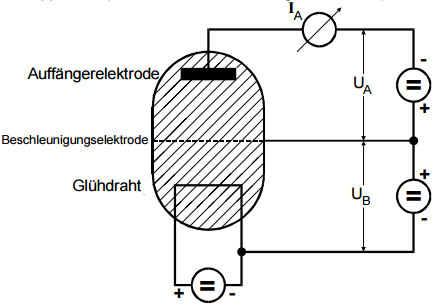
\includegraphics[height=7cm]{picture/Franck-Hertz-Apparatur}
  \caption{Schematischer Aufbau des Franck-Hertz-Versuches. \cite[2]{sample}}
  \label{fig:Apparatur}
\end{figure}

Die Apparatur besteht aus einem evakuierten Glasbehälter, in dem sich ein Glühdraht, eine Beschleunigerelektrode und eine Auffängerelektrode befindet. Außerdem befindet sich ein kleiner Tropfen Quecksilber in dem Glasbehälter. Der Glühdraht wird zur erzeugung von freien Elektronen verwendet und zwischen dem Glühdraht und der Beschleunigerelektrode liegt die Beschleunigungsspannung $U_\text{B}$ an. Diese Spannung beschleunigt die freien Elektronen in die Richtung der Auffängerelektrode. Die Bremsspannung $U_\text{A}$ liegt zwischen der Auffängerelektrode und der Beschleunigerelektrode an. Die Brems- und die Beschleunigungsspannung können sepparat voneinander durch jeweils ein konstant Spannungsgerät geregelt werden. Außerdem wird die Heizspannung auf einen konstanten Wert eingestellt. \\
Die für diesen Versuch verwendete Schaltung ist in Abbildung \eqref{fig:Schaltung} dargestellt.

\begin{figure}[H]
  \centering
  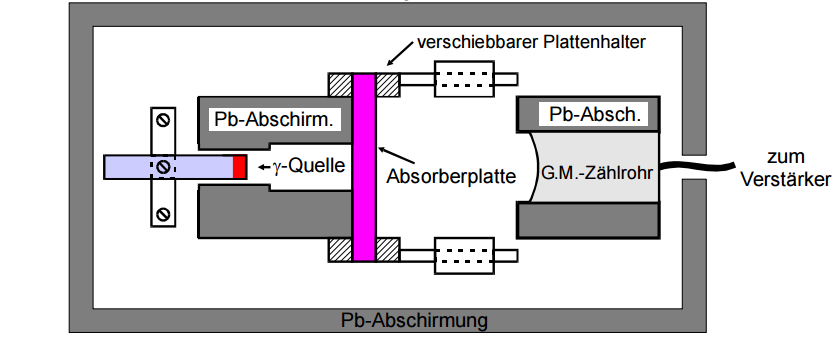
\includegraphics[height=5cm]{picture/Aufbau}
  \caption{Schaltung zur Aufnahme einer Franck-Hertz-Kurve}
  \label{fig:Schaltung}
\end{figure}

\subsection{Durchführung}
Dabei wird der Auffängerstrom $I_\text{A}$ von einem Picoamperemeter ausgelesen und auf den y-Eingang eines XY-Schreiber gegeben. 



























a
